\documentclass[A4,11pt]{article}
\usepackage[dvips]{graphicx}
\usepackage[spanish]{babel}
%\selectlanguage{spanish}
\usepackage[utf8]{inputenc}
\usepackage{amsthm,amsmath,amssymb,graphics,mathrsfs}
\usepackage[active]{srcltx}
\usepackage{hyperref}
\usepackage{cite}
\usepackage{multicol,pstricks,pstricks-add,setspace}
%\usepackage[margin=10pt,font=footnotesize,labelfont=bf,labelsep=endash]{caption}
\usepackage[left=4cm,top=3cm,right=2.4cm,bottom=3.2cm]{geometry}
% \newcolumntype{E}{>{$}c<{$}}
\usepackage{pst-all}
\usepackage{nonfloat}
\usepackage[bf,footnotesize]{caption2}
\usepackage{subfig}
\graphicspath{{C:/Users/USUARIO/Documents/GitHub/Proyecto\_Final\_EDP-NS/Gráficos/}}
\usepackage{caption}
\usepackage{subcaption}
\usepackage{wrapfig}
%\usepackage[dvips]{graphicx}
\pagestyle{myheadings}
\parindent=0pt
%opening
\usepackage{fancyhdr}
\pagestyle{fancy}
\fancyhead{}
\fancyhead[R]{Proyecto Modelado Matemático I}
\fancyfoot{}
\fancyfoot[L]{López, J. \textit{E-mail: \href{jorge2218061@correo.uis.edu.co}{jorge2218061@correo.uis.edu.co}}}
\fancyfoot[R]{\thepage}
\renewcommand{\headrulewidth}{0pt}
\title{{\huge \textbf{Buscando soluciones numéricas vía Python de EDPs: Una introducción de las EDPs en una y dos dimensiones que conducen a las ecuaciones de Navier-Stokes. }}}
\author{Jorge Leonardo López Agredo\\ 
	\small Universidad Industrial de Santander Escuela de Física\\
	 \small jorge2218061@correo.uis.edu.co\\ 
	\small Maestría en Matemática Aplicada\\
	 Docente: Ph.D Juan Carlos Basto Pineda\\ 
	\date{}
 }

\begin{document}

	\maketitle
	\vspace*{-1.5cm}
\begin{center}\rule{0.9\textwidth}{0.1mm} \end{center}

\section{Objetivo general}

Construir una actividad pedagógica para el curso de Modelado Matemático $I$, en el cual se introduzca las ideas básicas  de  los esquemas de diferencias finitas hacia adelante y hacia atrás, relacionadas con las soluciones numéricas de las ecuaciones diferenciales parciales vía Python.
\subsection{Objetivos específicos:}
\begin{enumerate}
	\item Crear un Jupyter Notebook donde se aborden la construcción de los esquemas de diferencias finitas que permita solucionar numéricamente una ecuación diferencial parcial en una dimensión.
	
	\item Desarrollar una actividad pedagógica que permita estudiar la ecuaciones en una dimensión necesarias para introducir las ecuaciones de Navier-Stokes.
	
	\item Introducir algunas ideas básicas para la construcción de un método numérico que permita afrontar el problema en dos dimensiones de las ecuaciones relacionadas con las ecuaciones de Navier-Stokes.
	
	\item  Diseñar un ejercicio final, donde los estudiantes puedan implementar las ideas desarrolladas en la actividad pedagógica, usando las herramientas aprendidas en el curso sobre Python y el esquema de diferencias finitas.

	
\end{enumerate}


%	\vspace*{-2.0cm}
\begin{center}\rule{0.9\textwidth}{0.1mm}
 \end{center}
\begin{multicols}{2}


\section{Introducción}

Las ecuaciones de Navier-Stokes (ENS) son un conjunto de ecuaciones diferenciales parciales (EDP) no lineales que describen el movimiento de un fluido viscoso, las cuales expresan matemáticamente la conservación de momento  y de la masa para los fluidos newtonianos (fluido cuya viscosidad puede considerarse constante)\cite{Achenson}.  Su nombre se debe en honor del físico e ingeniero francés Claude-Louis Navier (1785-1836) y al físico-matemático irlandés George Gabriel Stokes (1819-1903), los cuales desarrollaron la formulación integral y diferencial aplicando los principios de conservación de la mecánica y la termodinámica a un volumen de fluido y ciertas consideraciones como lo fue los esfuerzos tangenciales y su relación lineal con el gradiente de velocidad del movimiento del fluido, conocida como Ley de viscosidad de Newton\cite{Achenson}.\\


De las ENS no se dispone de una solución general de manera analítica, salvo para casos particulares, en fluidos específicos y bajo condiciones muy concretas\cite{Girault,Achenson}. Es por esto, que es preciso recurrir al análisis numérico, para determinar una solución aproximada que permita modelar problemas más generales. La dinámica de fluidos computacional (CFD) es la rama de la mecánica de fluidos que se ocupa del estudio mediante métodos numéricos de soluciones\cite{Barbagroup,Girault}.\\


En el desarrollo de este trabajo, el lector encontrará las ideas básicas que sustentan el marco teórico necesario, así como los esquemas de diferencias finitas para las simulaciones usadas en la discretización de las ecuaciones diferenciales que hemos a tratar en cada uno de los ejemplos propuestos. Seguidamente, se menciona el desarrollo pedagógico de cada uno de los notebooks. Para finalizar, se presenta algunas observaciones a modo de conclusión, producto del proceso realizado en las actividades propuestas \cite{LeonardoEC,LeonardoED,LeonardoEDP2d}).
\end{multicols}
\begin{center}\rule{0.9\textwidth}{0.1mm}
\end{center}
\begin{multicols}{2}
\section{Algunas ideas teóricas}

Las ecuaciones de Navier-Stokes están conformadas por un sistema de ecuaciones en derivadas parciales, las cuales describen el movimiento de un fluido viscoso incompresible. Se entiende por fluido a un agregado de partículas que se deforma en forma continua ante cualquier fuerza que actúe sobre él. La resistencia de un fluido a las deformaciones producidas por las tensiones corresponde a la viscosidad, y la incompresibilidad corresponde a la propiedad de algunos fluidos de preservar el volumen bajo efectos de presión.\\

Desde su formulación, en la primera mitad del siglo XIX, las ecuaciones de
Navier-Stokes han atraído el interés de muchos investigadores de la comunidad
científica mundial; ese interés se debe al hecho de que estas ecuaciones son
usadas en el estudio de problemas físicos relacionados con la metereología, la
aeronáutica, la oceanografía, la ingeniería hidráulica, entre otros, y también
desde el punto de vista matemático debido a la dificultad en el análisis cualitativo del
modelo y a una variedad de problemas abiertos que existen en la actualidad. En
efecto, es bien conocido que uno de los siete problemas del milenio, propuesto
por el Instituto Clay de Matemáticas, corresponde justamente con el problema de
existencia de solución global clásica de las ecuaciones de Navier-Stokes en el
caso tridimensional \cite{ClayM}.




 Para poder estudiar algunas ideas en la discretización de las ecuaciones que permiten tener una idea en el abordaje numérico de Navier-Stokes es importante comenzar estudiando la ecuación de convección lineal
\begin{equation}
	\label{ecl}
	\frac{\partial u}{\partial t} + c \frac{\partial u}{\partial x} = 0,
\end{equation}

con condiciones iniciales $u(x,0)=u_0(x)$, dato conocido como onda inicial. La ecuación representa la propagación de la onda inicial con velicidad $c$. La solución analítica usando variables separables es dada por $u(x,t)=u_0(x-ct)$. Para poder garantizar la existencia de las soluciones y la unicidad en algunos de los casos, de los problemas estudiados aquí, es importante usar resultados fuertes de Ecuaciones diferenciales parciales, para mayor imformación sobre esto vease por ejemplo \cite{Girault}.\\

Finalmente, las ecuaciones de Navier-Stokes para un fluido incompresible, 

\begin{equation}
	\label{edNavierStokes}
	\begin{split}
	\nabla \cdot\vec{v} &= 0 \\
	\frac{\partial \vec{v}}{\partial t}+(\vec{v}\cdot\nabla)\vec{v} &= -\frac{1}{\rho}\nabla p + \nu \nabla^2\vec{v},
	\end{split}
\end{equation}

donde $\vec{v}$ representa el campo de velocidades del fluido, $\rho$ la densidad del fluido, $p$ la presión y $\nu$ es el coeficiente de viscocidad del fluido. Hasta el momento, desde el punto de vista analítico, se conocen dos maneras de enfrentar el problema de Cauchy
asociado a las ecuaciones de Navier-Stokes. La primera de ellas es debida a
Jean LERAY \cite{leray} quien introdujo el concepto de soluciones débiles (turbulentas), y la segunda es debida a Tosio KATO \cite{kato} que permite obtener la existencia y unicidad de soluciones (blandas) globales y regulares, bajo condiciones
de pequeñez de los datos iniciales y de las fuerzas externas que actúan sobre
el fluido. El concepto de solución débil introducido por Leray permite el análisis
de soluciones en espacios mas grandes a los espacios clásicos para describir el
movimiento de un fluido; más aún, una de las motivaciones planteadas por Leray
era la de considerar una clase de soluciones permitiendo que el rotacional de la
velocidad tienda a infinito en tiempo finito.\\

Es por esto, que nos vemos motivamos a adentrarnos en el maravilloso mundo de las aproximaciones de las soluciones para EDPs desde el punto de vista numérico. Y que mejor manera de hacerlo, que estudiando las ecuaciones previas en las cuales se sustenta las ENS, sus discretizaciones para poder implemetar códigos que nos permitan buscar soluciones numéricas y poder visualizar algunos detalles básicos para entender de que va todo esto, al buscar soluciones numéricas vía Python de EDPs.\\

 Como observaciones finales, la primera ecuación representa la conservación de la masa cuando la densidad es constante. La segunda ecuación es la conservación del momento. Pero aparece un problema: la ecuación de continuidad para el flujo incompresible $ \nabla \cdot \vec{v} = 0 $ no tiene una variable dominante y no hay una forma obvia de acoplar la velocidad  y la presión $ p $. En el caso del flujo compresible, por el contrario, la continuidad de la masa proporcionaría una ecuación de evolución para la densidad $ \rho $, que se acopla con una ecuación de estado que relaciona $ \rho $ y $ p $. Para ello, debemos hacer un estudio de discretización de la ecuación de Poisson 2-D
$$\frac{\partial ^2 p}{\partial x^2} + \frac{\partial ^2 p}{\partial y^2} = b,$$
donde si $b=0$ se conoce como la ecuación de Laplace.


\end{multicols}
\begin{center}\rule{0.9\textwidth}{0.1mm}
\end{center}
\begin{multicols}{2}
	
\section{Desarrollo Pedagógico}

Para el desarrollo de la actividad pedagógica se desarrolla en dos secciones, en las cuales se desarrollan actividades que involucan la creación de los métodos numéricos que discretizan las siguientes ecuaciones diferenciales parciales(Ver \cite{LeonardoEC,LeonardoED,LeonardoEDP2d})

\begin{enumerate}
	\item Ecuación de convección lineal 1-D.
	\item Ecuación de convección no lineal 1-D.
	\item Ecuación de difusion 1-D.
	\item Ecuación de Burgers 1-D.
	\item Ecuación de convección lineal 2-D, ecuación de difusión 2-D, sistemas de ecuaciones no lineales acopladas y Ecuación de Burgers 2-D.
\end{enumerate}
La teoría que sustenta cada uno de los procesos de discretización así como los métodos numéricos usados para poder definir las discretizaciones de cada una de las EDPs estudiadas se encuentran dentro de los Jupyter Notebooks desarrollados para esta actividad \cite{LeonardoEC,LeonardoED,LeonardoEDP2d}, los cuales están basados en el trabajo realizado de la PhD Lorena A. Barba @LorenaABarba, quien desarrolló el material CFDPython \cite{Barba,Barbagroup}, sobre el cual está desarrollado el siguiente proyecto pedagógico. Adicionalmente, de planean actividades para desarrollo personalizado que permitan reforzar y caracterizar los conceptos alcanzados durante las secciones. \\

Para poder implementar el método numérico para las EDPs a estudiar, como por ejemplo \ref{ecl}, nosotros discretizamos esta ecuación tanto en el tiempo como en el espacio, usando el esquema de diferencias finitas hacia adelante\cite{Barbagroup,Girault} para la derivada en el tiempo y el esquema de diferencias finitas hacia atrás\cite{Barbagroup,Girault} para la derivada en el espacio. La coordenada espacial $x$ se discretiza en $N$ pasos regulares $\Delta x$ desde $i=0$ hasta $i=N$. Para la variable temporal $t$ se discretiza tomando intervalos de tamaño $\Delta t$.\\
Por la definición de derivada, removiendo el límite, es posible aproximar
$$\frac{\partial u}{\partial x}\approx \frac{u(x+\Delta x)-u(x)}{\Delta x}.$$

Así, por nuestra discretización, se sigue que:
$$\frac{u_i^{n+1}-u_i^n}{\Delta t} + c \frac{u_i^n - u_{i-1}^n}{\Delta x} = 0, $$
donde $n$ y $n+1$ son dos pasos en el tiempo, mientras que $i-1$ y $i$ son dos puntos vecinos de la coodenada $x$ discretizada. Si se tienen en cuenta la condiciones iniciales, la única variable desconocida es $u_i^{n+1}$. Resolviendo la ecuación para $u_i^{n+1}$, podemos obtener una ecuación que nos permita avanzar en el tiempo de la siguiente manera: 
\begin{tiny}
\begin{equation}
	\label{decl}
	u_i^{n+1} = u_i^n - c \frac{\Delta t}{\Delta x}(u_i^n-u_{i-1}^n).
\end{equation}
\end{tiny}
De manera análoga, es posible discretizar la ecuación lineal de convección 2-D
\begin{equation}
	\label{ecl2d}
	\frac{\partial u}{\partial t}+c\frac{\partial u}{\partial x} + c\frac{\partial u}{\partial y} = 0,
\end{equation}

como se sigue:
\begin{tiny}
\begin{equation}
	\label{decl2d}
	u_{i,j}^{n+1} = u_{i,j}^n-c \frac{\Delta t}{\Delta x}(u_{i,j}^n-u_{i-1,j}^n)-c \frac{\Delta t}{\Delta y}(u_{i,j}^n-u_{i,j-1}^n).
\end{equation}	
\end{tiny}

Ahora, es posible estudiar la ecuación de convección no lineal 1-D 
\begin{equation}
	\label{ecnl}
	\frac{\partial u}{\partial t} + u \frac{\partial u}{\partial x} = 0,
\end{equation}

y discretizarla mediante:

\begin{tiny}
\begin{equation}
	\label{decnl}
	u_i^{n+1} = u_i^n - u_i^n \frac{\Delta t}{\Delta x} (u_i^n - u_{i-1}^n).
\end{equation}
	
\end{tiny}

Generalizar esta idea a 2-D nos permite obtener un sistema de dos EDP no lineales acopladas, relacionadas así:
\begin{equation}
	\label{ecnl2d}
	\begin{split}
		\frac{\partial u}{\partial t} + u \frac{\partial u}{\partial x} + v \frac{\partial u}{\partial y} &= 0,\\	
		\frac{\partial v}{\partial t} + u \frac{\partial v}{\partial x} + v \frac{\partial v}{\partial y} &= 0.
	\end{split}
\end{equation}


Cuya discretización se define como:

\begin{tiny}
	\begin{equation}
		\label{decnl2d}
		\begin{split}
			u_{i,j}^{n+1} &= u_{i,j}^n - u_{i,j} \frac{\Delta t}{\Delta x} (u_{i,j}^n-u_{i-1,j}^n) - v_{i,j}^n \frac{\Delta t}{\Delta y} (u_{i,j}^n-u_{i,j-1}^n),\\	
			v_{i,j}^{n+1} &= v_{i,j}^n - u_{i,j} \frac{\Delta t}{\Delta x} (v_{i,j}^n-v_{i-1,j}^n) - v_{i,j}^n \frac{\Delta t}{\Delta y}
			(v_{i,j}^n-v_{i,j-1}^n).
		\end{split}
	\end{equation}
\end{tiny}

Ideas análogas a las descritas anteriormente, nos permiten afrontar otras EDP importantes en el objetivo de poder encontrar soluciones numéricas para las ENS. Entre ellas se destacan la ecuación de difusión 1-D 
\begin{equation}
	\label{ed}
	\frac{\partial u}{\partial t}= \nu \frac{\partial^2 u}{\partial x^2}
\end{equation}

y su generalización a 2-D.
\begin{equation}
	\label{ed2d}
	\frac{\partial u}{\partial t} = \nu \frac{\partial ^2 u}{\partial x^2} + \nu \frac{\partial ^2 u}{\partial y^2}.
\end{equation}
Cuyas discretizaciones se siguen de manera natural al considerar el desarrollo en series mediante el teorema de Taylor( ver \cite{LeonardoED, LeonardoEDP2d}). La derivada de segundo orden se puede representar geométricamente como la línea tangente a la curva dada por la primera derivada. Discretizaremos la derivada de segundo orden con un esquema de Diferencia Central: una combinación de Diferencias hacia adelante y Diferencias hacia atrás de la primera derivada. Considere la expansión de Taylor de $ u_{i + 1} $ y $ u_{i-1} $ alrededor de $ u_i $:

\begin{tiny}
\begin{equation*}
	\begin{split}
		u_{i+1} &= u_i + \Delta x \frac{\partial u}{\partial x}\bigg|_i + \frac{\Delta x^2}{2} \frac{\partial ^2 u}{\partial x^2}\bigg|_i + \frac{\Delta x^3}{3!} \frac{\partial ^3 u}{\partial x^3}\bigg|_i + O(\Delta x^4).\\
		u_{i-1} &= u_i - \Delta x \frac{\partial u}{\partial x}\bigg|_i + \frac{\Delta x^2}{2} \frac{\partial ^2 u}{\partial x^2}\bigg|_i - \frac{\Delta x^3}{3!} \frac{\partial ^3 u}{\partial x^3}\bigg|_i + O(\Delta x^4).
	\end{split}	
\end{equation*}	
\end{tiny}

Así, 
$$\frac{\partial ^2 u}{\partial x^2}=\frac{u_{i+1}-2u_{i}+u_{i-1}}{\Delta x^2} + O(\Delta x^4)$$

de donde se obtiene, la discretización de la ecuación de difusión 1-D \ref{ed}
\begin{tiny}
\begin{equation}
	\label{ded}
	u_{i}^{n+1}=u_{i}^{n}+\frac{\nu\Delta t}{\Delta x^2}(u_{i+1}^{n}-2u_{i}^{n}+u_{i-1}^{n}),	
\end{equation}	
\end{tiny}

y, la discretización de manera natural de su generalización a 2-D \ref{ed2d} es dada por 
\begin{tiny}
\begin{equation}
	\label{ded2d}
	\begin{split}
		u_{i,j}^{n+1} = u_{i,j}^n &+ \frac{\nu \Delta t}{\Delta x^2}(u_{i+1,j}^n - 2 u_{i,j}^n + u_{i-1,j}^n) \\
		&+ \frac{\nu \Delta t}{\Delta y^2}(u_{i,j+1}^n-2 u_{i,j}^n + u_{i,j-1}^n)
	\end{split}	
\end{equation}	
\end{tiny}

La ecuación de Burgues (EB) en una dimensión espacial, es una combinación de la ecuación de convección no lineal y la ecuación de difusión (Ver por ejemplo \cite{LeonardoED}). La generalización de esta en 2-D, es dada por:

\begin{equation}
	\label{eb2d}
	\begin{split}
		\frac{\partial u}{\partial t} + u \frac{\partial u}{\partial x} + v \frac{\partial u}{\partial y} &= \nu \; \left(\frac{\partial ^2 u}{\partial x^2} + \frac{\partial ^2 u}{\partial y^2}\right)\\
		\frac{\partial v}{\partial t} + u \frac{\partial v}{\partial x} + v \frac{\partial v}{\partial y} &= \nu \; \left(\frac{\partial ^2 v}{\partial x^2} + \frac{\partial ^2 v}{\partial y^2}\right).
	\end{split}
\end{equation}

Se resalta entre las actividades desarrolladas el uso de la librería \textbf{SymPy} la cual es la biblioteca matemática simbólica de Python. Tiene muchas de las mismas funciones matemáticas simbólicas que Mathematica con el beneficio adicional de que podemos traducir fácilmente sus resultados a nuestros cálculos de Python (también es gratuito y de código abierto). Por otra parte, se hace uso de las librerías \textbf{mpl\_toolkits.mplot3d} y \textbf{matplotlib} para el desarrollo y representación de buenos gráficos que permitan ilustrar algunas caracteristicas de las soluciones de las EDPs.  
\end{multicols}
\begin{center}\rule{0.9\textwidth}{0.1mm}
\end{center}
\section{Observaciones finales}
Como parte final de esta disertación, se presentan algunos resultados gráficos de los resultados obtenidos tanto en 1-D como en 2-D de aplicar los métodos numéricos al buscar soluciones del problema de Cauchy con dato inicial $u(x,0)=u_0(x)$ en el intervalo de tiempo $[0,2]$, mostrada en la figura \ref{dato_inicial} para los problemas 1-D, y en la figura \ref{dato_inicial2d} para el caso 2D.\\

\begin{wrapfigure}{r}{0.40\textwidth} %this figure will be at the right
	\centering
	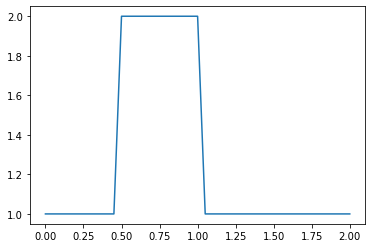
\includegraphics[width=0.30\textwidth]{dato_inicial.png}
	\caption[]{$u_0(x)$ en 2-D}
		\label{dato_inicial}
\end{wrapfigure}
En el desarrollo de de cada uno de los notebooks se parte de una información conocida como onda inicial o dato inicial $u(x,0)=u_0(x)$, y vamos a tomar una onda que suele ser importante en la teoría de fluidos, conocida como onda de choque, la cual se define para el caso 1-D, como $ u = 2 $ en el intervalo $ 0.5 \leq x \leq 1 $ y $ u = 1 $ en cualquier otro lugar de $ (0,2) $ (es decir, una función de sombrero). \\

\begin{wrapfigure}{l}{0.35\textwidth} %this figure will be at the right
	\centering
	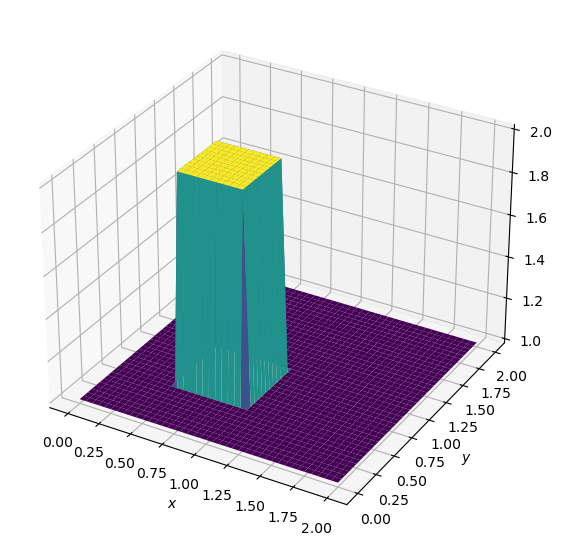
\includegraphics[width=0.30\textwidth]{dato_inicial_2D.png}
	\caption[]{ $u_0(x)$ en 2-D}
	\label{dato_inicial2d}
\end{wrapfigure}
De manera análoga, para el caso 2-D, se tiene que
$$u, v = \begin{cases}\begin{matrix}
		2 & \text{para } x,y \in (0.5, 1)\times(0.5,1) \cr
		1 & \text{c.c}
\end{matrix}\end{cases}$$
 con condiciones de contorno dadas por 
 $$u = 1,\ v = 1 \text{ para } \begin{cases} \begin{matrix}x=0,2\cr y=0,2 \end{matrix}\end{cases}$$

 Al analizar la ecuación de convección lineal y no lineal con dato inicial $u_0$ para diferentes refinamientos $nx$, podemos ver lo el desplazamiento de la onda, como una translación rígida en el eje $x$, de $ct$ unidades hacia la derecha(Ver Figura \ref{sol_ecl}).
\begin{figure}[h]
	\centering
	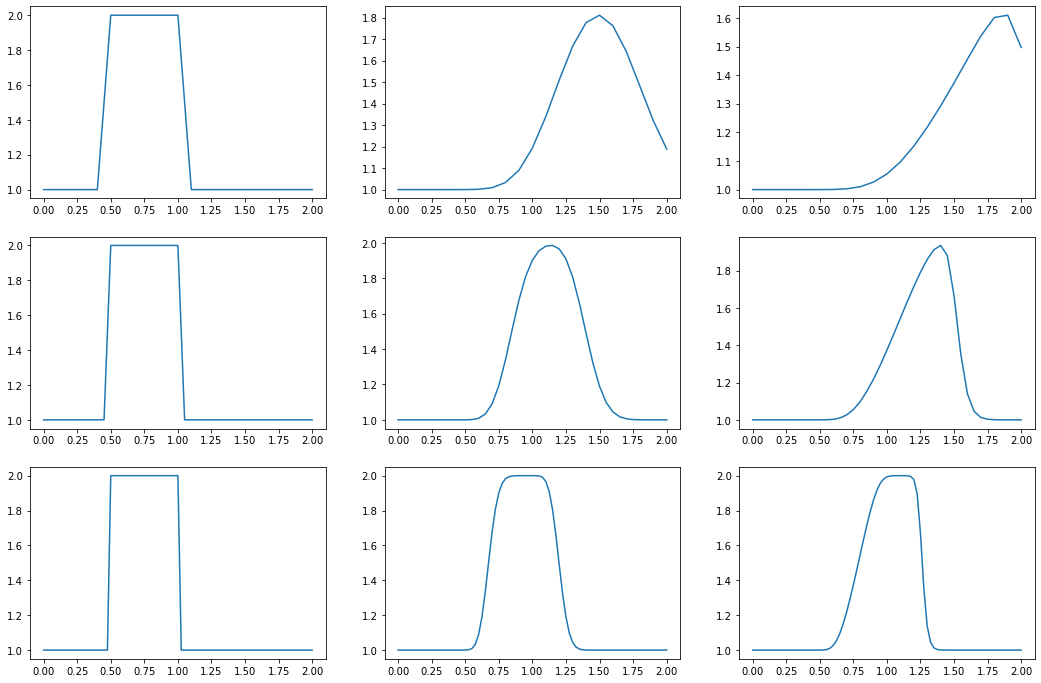
\includegraphics[width=0.65\textwidth]{sol_ecl_ecnl.png}
	\caption{Comparación entre la solución de la ecuación de convección lineal vs ecuación de convección no lineal}
	\label{sol_ecl}
\end{figure}

 En esta figura, tenemos la primera fila presenta el dato inicial, la solución al problema lineal y la solución al problema no lineal, en su orden para $nx = 21$. De manera análoga, la segunda fila es para $nx = 41$ y la tercera es para $nx=81$. Donde cabe la pena resaltar que se ha tenido en cuenta para la convergencia del modelo, la definición $\sigma$, conocida como número de Courant (CFL) \cite{Achenson}.
 
 Finalmente, mostramos la evolución en tiempo para la solución de la ecuación de Difusión en 2-D (Ver Figura \ref{sol_ed}), para el dato inicial $u_0$, en el cual se evidencia el fenómeno físico, y podemos compararla con el la ecuación de Burges 2-D (Ver Figura \ref{sol_eb}). 
 
 \begin{figure}[h]
	\centering
	\subfloat[$t=0.5$]{
		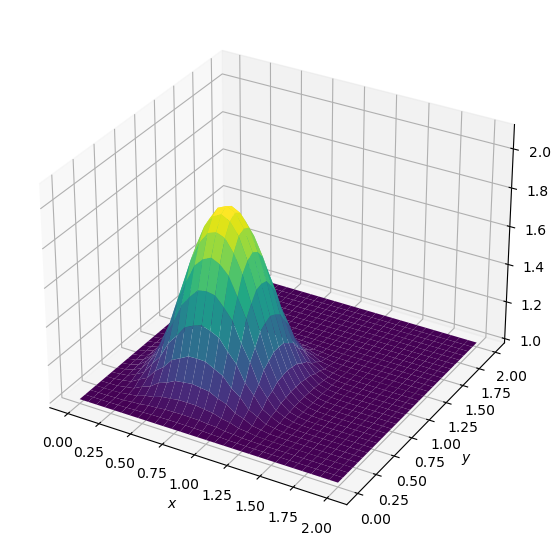
\includegraphics[width=0.3\textwidth]{sol_ed_2D_1.png}}	
	\subfloat[$t=1$]{
		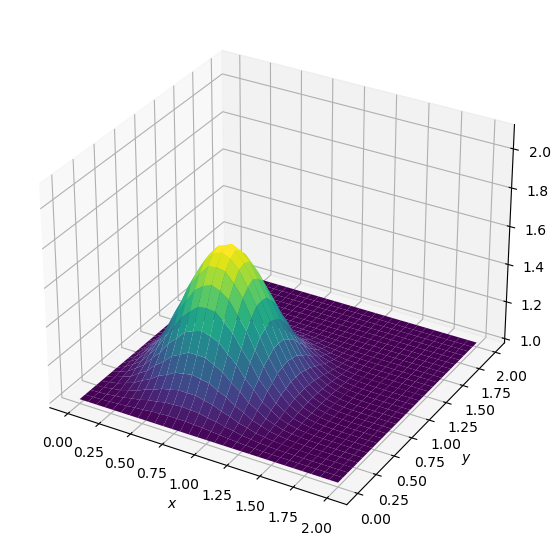
\includegraphics[width=0.3\textwidth]{sol_ed_2D_2.png}}	
	\subfloat[$t=2$]{
		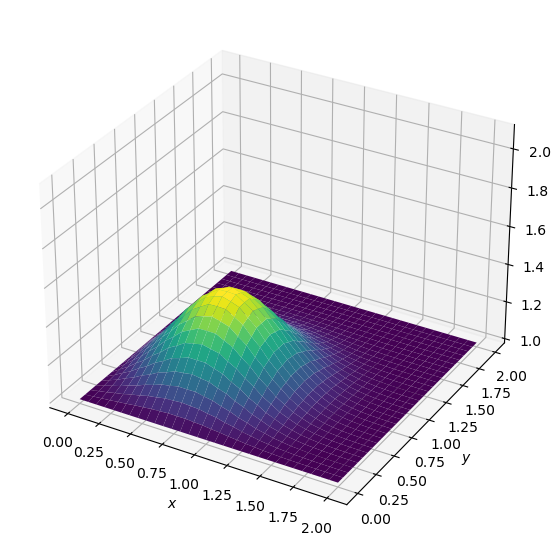
\includegraphics[width=0.3\textwidth]{sol_ed_2D_3.png}}
	\caption{Soluciones para diferentes $t$ de la Ecuación de Difusion 2-D \ref{ed2d}}
	\label{sol_ed}
\end{figure}

Es interesante resaltar, el comportamiento de un mismo dato inicial, sujeto a condiciones de entorno diferentes, en especial si tenemos modelos que representan no solo problemas de difusión sino  que incluyan una ley de transporte.\\

\begin{figure}[h]
	\centering
	\subfloat[$t=0.5$]{
		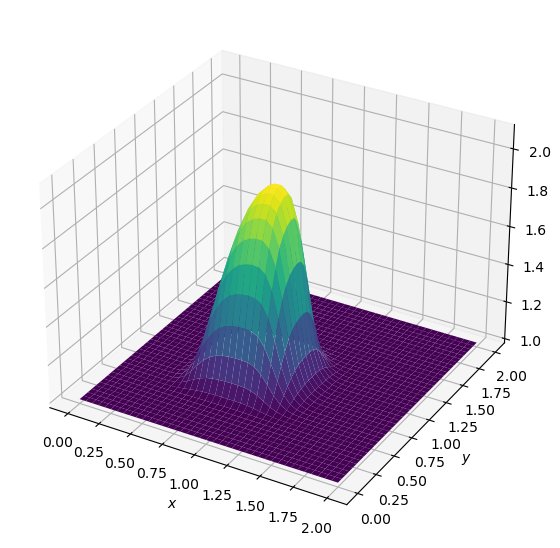
\includegraphics[width=0.3\textwidth]{sol_eb_2D_1.png}}	
	\subfloat[$t=1$]{
		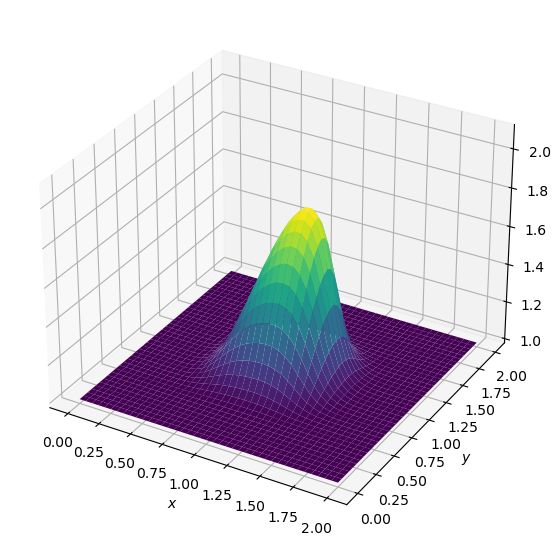
\includegraphics[width=0.3\textwidth]{sol_eb_2D_2.png}}	
	\subfloat[$t=2$]{
		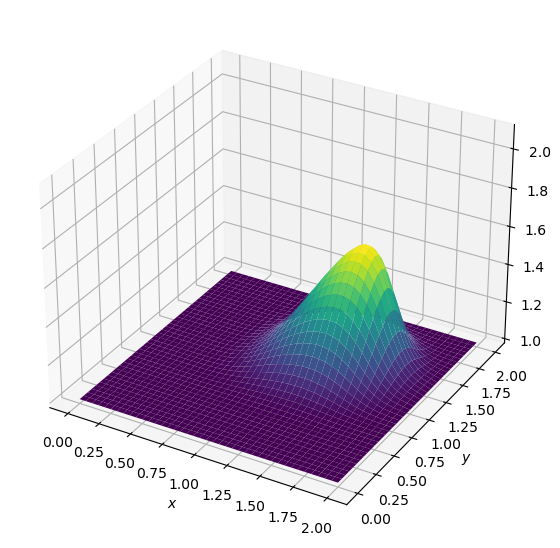
\includegraphics[width=0.3\textwidth]{sol_eb_2D_3.png}}
	\caption{Soluciones para diferentes $t$ de la Ecuación de Burgers 2-D \ref{eb2d}}
	\label{sol_eb}
\end{figure}


Para finalizar el presente trabajo, se agradece de manera puntual el compromiso del docente del área y los conocimientos adquiridos durante el semestre para poder afrontar los retos que se avecinan, y más aún, dotarnos de herrramientas básicas y necesarias para el estudio y las futuras investigaciones. Hoy no es posible hablar de investigación si no tenemos herramientas de computación que nos permita modelar, simular y comparar los resultados teóricos con los experimentales. Este fue uno de los grandes objeticos, y era el ver la potencia y congruencia del metodo, con la realidad teórica y analítica de las soluciones a problemas, que se pueden convertir, mejorar y expandir a cuestiones más robustas y aplicadas a la actualidad y a la necesidad del investigador.
\begin{center}\rule{0.9\textwidth}{0.1mm}
\end{center}
\begin{thebibliography}{99}
	\addcontentsline{toc}{chapter}{Bibliografía}
\bibitem{ClayM} Clay Mathematics Institute. Navier–Stokes Equation. [en linea]. (Recuperado en 24 de febrero de 2018). Disponible en \href{http://www.claymath.org/millennium-problems/navier-stokes-equation.}{http://www.claymath.org/millennium-problems/navier-stokes-equation}.
	\bibitem{Barba} Barba, Lorena A., and Forsyth, Gilbert F. (2018). \textit{CFD Python: the 12 steps to Navier-Stokes equations}. Journal of Open Source Education, 21. [\href{https://doi.org/10.21105/jose.00021}{https://doi.org/10.21105/jose.00021}]
	
		\bibitem{LeonardoEC} López, L. (2021) \textit{Proyecto\_Final\_EDP-NS}.\href{https://github.com/LeonardoLopez2218061/Proyecto_Final_EDP-NS/blob/main/Desarrollo_Jupyter/ecuacion_conveccion.ipynb}{ecuacion\_conveccion.ipynb}
%\bibitem{sch1} SCHRÖDINGER , E. \textit{Annalen der Physik ILXXX}. Folge 361, 1926.
%\bibitem{opticalphysics} LIPSON, S. G.; LIPSON, H. \textit{Optical Physics.} 2 ed. New York: Cambridge University Press, 1981.
%\bibitem{mediblefuncion} S. LUNDEEN, J. S.; SUTHERLAND, B.; PATELL, A.;  STEWART C. \&  BAMBERT, C. \emph{Direct measurement of the quantum wavefunction.} Nature 474, (2011). p. 188-191.
\bibitem{Barbagroup} Barbagroup, (2019). \textit{CFDPython}. [\href{https://github.com/barbagroup/CFDPython}{https://github.com/barbagroup/CFDPython}]
\bibitem{Achenson} Achenson, D. J. (1990). \textit{Elementary Fluid Dynamics, Oxford Applied Mathematics and Computing Science Series}. Oxford University Press, ISBN 0-19-859679-0.
	\bibitem{LeonardoED} López, L. (2021) \textit{Proyecto\_Final\_EDP-NS}. [\href{https://github.com/LeonardoLopez2218061/Proyecto_Final_EDP-NS/blob/main/Desarrollo_Jupyter/ecuacion_difusion_and_burguers.ipynb}{ecuacion\_difusion\_and\_burguers.ipynb}]
\bibitem{Girault} V. Girault and P.A. Raviart. \textit{Finite Element Methods for Navier–Stokes Equations: Theory and Algorithms}. Springer Series in Computational Mathematics. Springer-Verlag, 1986.
\bibitem{kato} Kato, T. (1984). Strong $L^{p}(\mathbb{R}^n)$ solutions of the Navier–Stokes equations in $\mathbb{R}^n$ with applications, Math. Z., 187, 471-480.
\bibitem{leray} ] Leray, J. (1933). Etude de diverses équations intégrales non linéaires et de quelques problémes que pose l’hydrodynamique, J. Math. Pures Appl, 12, 1-82.
	\bibitem{LeonardoEDP2d} López, L. (2021) \textit{Proyecto\_Final\_EDP-NS}. [\href{https://github.com/LeonardoLopez2218061/Proyecto_Final_EDP-NS/blob/main/Desarrollo_Jupyter/trabajandoEDP_en_2D.ipynb}{trabajandoEDP\_en\_2D.ipynb}]

\end{thebibliography}
\end{document}
